\documentclass{beamer}
\usetheme{default}
\usecolortheme{default}
\setbeamertemplate{navigation symbols}{}

\usepackage{tikz}
\usetikzlibrary{positioning, fit, backgrounds, arrows.meta}

\definecolor{devcol}{RGB}{70, 130, 180}
\definecolor{rescol}{RGB}{210, 105, 30}

\tikzset{
  block/.style={draw, rounded corners, minimum width=2.6cm, minimum height=0.7cm,
                align=center, font=\small},
  flow/.style={-{Latex[length=2.5mm]}, thick},
}

\title{Signal Processing Framework}
\subtitle{Real-time and offline audio processing in Python}
\author{Noam Shabtai}
\date{}

\begin{document}

\frame{\titlepage}

% ------------------------------------------------------------------
\begin{frame}{Architecture}
\centering
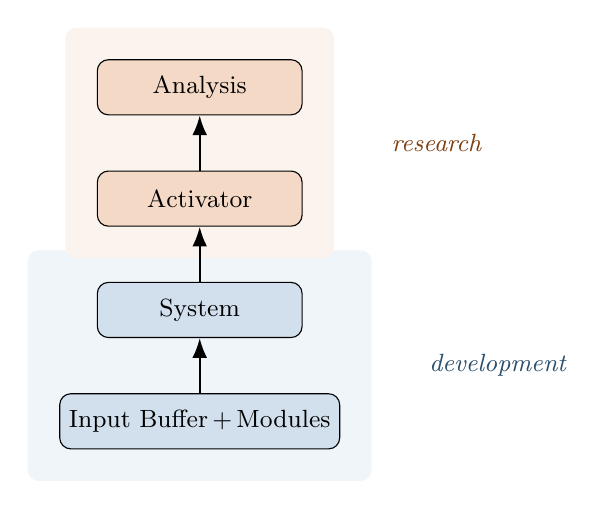
\begin{tikzpicture}[node distance=0.7cm]
  \node[block, fill=devcol!25]                (bm)  {Input Buffer\,+\,Modules};
  \node[block, fill=devcol!25, above=of bm]   (sys) {System};
  \node[block, fill=rescol!25, above=of sys]  (act) {Activator};
  \node[block, fill=rescol!25, above=of act]  (ana) {Analysis};

  \draw[flow] (bm)  -- (sys);
  \draw[flow] (sys) -- (act);
  \draw[flow] (act) -- (ana);

  \begin{scope}[on background layer]
    \node[fill=devcol!8, fit=(bm)(sys), rounded corners, inner sep=4mm] (devband) {};
    \node[fill=rescol!8, fit=(act)(ana), rounded corners, inner sep=4mm] (resband) {};
  \end{scope}

  \node[right=0.6cm of devband, font=\small\itshape, text=devcol!60!black] {development};
  \node[right=0.6cm of resband, font=\small\itshape, text=rescol!60!black] {research};
\end{tikzpicture}
\end{frame}

% ------------------------------------------------------------------
\begin{frame}{Input Buffer \& Modules}
\centering
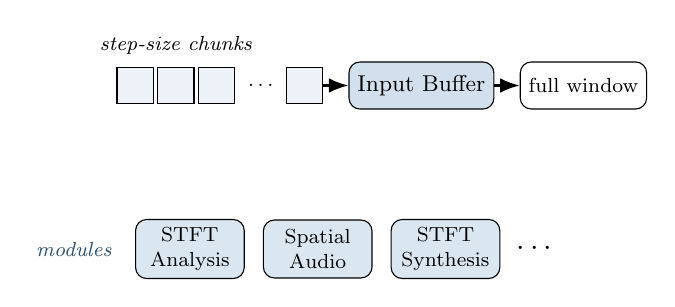
\begin{tikzpicture}[node distance=0.4cm, scale=0.92, transform shape]
  % --- Input Buffer row ---
  \node[font=\footnotesize, minimum width=0.5cm, minimum height=0.5cm,
        draw, fill=devcol!10] (c1) {};
  \node[font=\footnotesize, minimum width=0.5cm, minimum height=0.5cm,
        draw, fill=devcol!10, right=0.05cm of c1] (c2) {};
  \node[font=\footnotesize, minimum width=0.5cm, minimum height=0.5cm,
        draw, fill=devcol!10, right=0.05cm of c2] (c3) {};
  \node[font=\footnotesize, right=0.05cm of c3] (cdots) {$\cdots$};
  \node[font=\footnotesize, minimum width=0.5cm, minimum height=0.5cm,
        draw, fill=devcol!10, right=0.05cm of cdots] (cn) {};
  \node[font=\footnotesize\itshape, above=0.05cm of c2] {step-size chunks};

  \node[block, fill=devcol!25, right=0.35cm of cn, minimum width=2cm, minimum height=0.65cm] (ib) {Input Buffer};
  \draw[flow] (cn) -- (ib);

  \node[block, fill=white, right=0.35cm of ib, font=\footnotesize, minimum width=1.5cm, minimum height=0.65cm] (win) {full window};
  \draw[flow] (ib) -- (win);

  % --- Modules row ---
  \node[block, fill=devcol!20, below=2cm of c1, anchor=west,
        font=\footnotesize, minimum width=1.5cm, minimum height=0.8cm] (m1) {STFT\\Analysis};
  \node[block, fill=devcol!20, right=0.25cm of m1,
        font=\footnotesize, minimum width=1.5cm, minimum height=0.8cm] (m2) {Spatial\\Audio};
  \node[block, fill=devcol!20, right=0.25cm of m2,
        font=\footnotesize, minimum width=1.5cm, minimum height=0.8cm] (m3) {STFT\\Synthesis};
  \node[font=\large, right=0.1cm of m3] (mdots) {$\cdots$};

  \node[font=\footnotesize\itshape, text=devcol!60!black,
        left=0.2cm of m1, anchor=east] {modules};
\end{tikzpicture}

\vspace{0.7cm}
\footnotesize
\begin{tabular}{ll}
\textbf{Input Buffer} & accumulates step-size chunks until a window is ready \\
\textbf{Modules}      & independent signal processors (frequency or time domain) \\
\end{tabular}
\end{frame}

% ------------------------------------------------------------------
\begin{frame}{System}
\centering
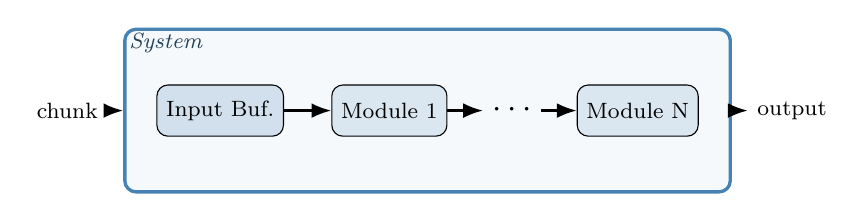
\begin{tikzpicture}[node distance=0.6cm]
  \node[block, fill=devcol!25, font=\footnotesize, minimum width=1.3cm, minimum height=0.65cm] (ib) {Input Buf.};
  \node[block, fill=devcol!20, right=of ib, font=\footnotesize, minimum width=1.2cm, minimum height=0.65cm] (m1) {Module 1};
  \node[font=\large, right=0.45cm of m1] (dots) {$\cdots$};
  \node[block, fill=devcol!20, right=0.45cm of dots, font=\footnotesize, minimum width=1.2cm, minimum height=0.65cm] (mn) {Module N};

  \draw[flow] (ib)   -- (m1);
  \draw[flow] (m1)   -- (dots);
  \draw[flow] (dots) -- (mn);

  \begin{scope}[on background layer]
    \node[draw=devcol, very thick, rounded corners, fill=devcol!5,
          fit=(ib)(mn), inner xsep=4mm, inner ysep=7mm] (sys) {};
  \end{scope}
  \node[font=\footnotesize\itshape, text=devcol!50!black,
        anchor=north west, inner sep=2pt] at (sys.north west) {System};

  \node[font=\footnotesize, left=0.2cm of sys] (inarr) {chunk};
  \draw[flow] (inarr) -- (sys);
  \node[font=\footnotesize, right=0.2cm of sys] (outarr) {output};
  \draw[flow] (sys) -- (outarr);
\end{tikzpicture}

\vspace{0.8cm}
\small
\textbf{System} calls each module's \texttt{execute()} and connects
the output of one module to the input of the next.
\end{frame}

% ------------------------------------------------------------------
\begin{frame}{Offline Activator}
\centering
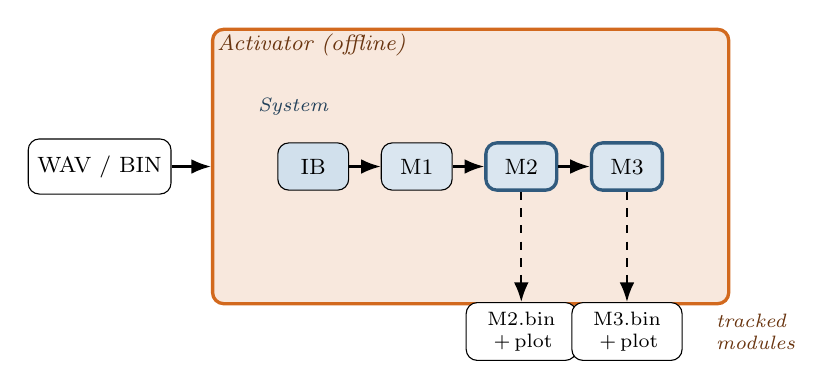
\begin{tikzpicture}[node distance=0.4cm]
  \node[block, fill=devcol!25, font=\footnotesize, minimum width=0.9cm, minimum height=0.6cm] (ib) {IB};
  \node[block, fill=devcol!20, right=of ib, font=\footnotesize, minimum width=0.9cm, minimum height=0.6cm] (m1) {M1};
  \node[block, fill=devcol!20, draw=devcol!70!black, very thick,
        right=of m1, font=\footnotesize, minimum width=0.9cm, minimum height=0.6cm] (m2) {M2};
  \node[block, fill=devcol!20, draw=devcol!70!black, very thick,
        right=of m2, font=\footnotesize, minimum width=0.9cm, minimum height=0.6cm] (m3) {M3};

  \draw[flow] (ib) -- (m1);
  \draw[flow] (m1) -- (m2);
  \draw[flow] (m2) -- (m3);

  \begin{scope}[on background layer]
    \node[draw=devcol, very thick, rounded corners, fill=devcol!8,
          fit=(ib)(m3), inner xsep=3mm, inner ysep=6mm] (sys) {};
  \end{scope}
  \node[font=\scriptsize\itshape, text=devcol!50!black,
        anchor=north west, inner sep=2pt] at (sys.north west) {System};

  \begin{scope}[on background layer]
    \node[draw=rescol, very thick, rounded corners, fill=rescol!15,
          fit=(sys), inner xsep=5mm, inner ysep=8mm] (act) {};
  \end{scope}
  \node[font=\footnotesize\itshape, text=rescol!50!black,
        anchor=north west, inner sep=2pt] at (act.north west) {Activator (offline)};

  \node[block, fill=white, font=\footnotesize, align=center,
        left=0.5cm of act, minimum width=1.5cm] (in) {WAV / BIN};
  \draw[flow] (in) -- (act);

  \node[block, fill=white, font=\scriptsize, align=center,
        below=1.4cm of m2, minimum width=1.4cm] (out2) {M2.bin\\\,+\,plot};
  \node[block, fill=white, font=\scriptsize, align=center,
        below=1.4cm of m3, minimum width=1.4cm] (out3) {M3.bin\\\,+\,plot};

  \draw[flow, dashed] (m2) -- (out2);
  \draw[flow, dashed] (m3) -- (out3);

  \node[font=\scriptsize\itshape, text=rescol!50!black,
        right=0.3cm of out3, anchor=west, align=left] {tracked\\modules};
\end{tikzpicture}

\vspace{0.7cm}
\footnotesize
\begin{tabular}{ll}
\textbf{Offline Activator} & file-to-file batch processor \\
                           & \texttt{execute()} runs the full chunk loop synchronously \\
                           & saves one \texttt{.bin} per \emph{tracked module} of the system \\
                           & + optional PNG plot per tracked module \\
\end{tabular}
\end{frame}

% ------------------------------------------------------------------
\begin{frame}{Demo Activator}
\centering
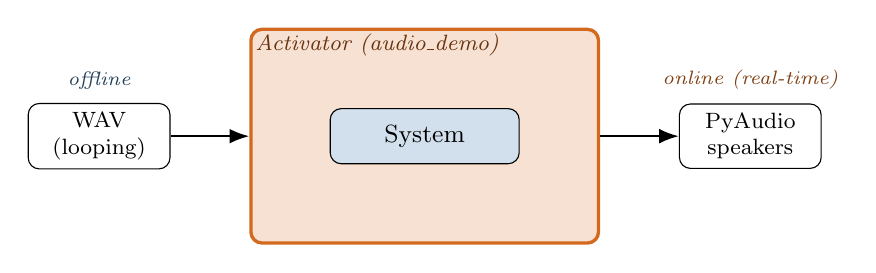
\begin{tikzpicture}[node distance=0.5cm]
  \node[block, fill=devcol!25, minimum width=2.4cm] (sys) {System};

  \begin{scope}[on background layer]
    \node[draw=rescol, very thick, rounded corners, fill=rescol!20,
          fit=(sys), inner xsep=10mm, inner ysep=10mm] (act) {};
  \end{scope}
  \node[font=\footnotesize\itshape, text=rescol!50!black,
        anchor=north west, inner sep=2pt] at (act.north west) {Activator (audio\_demo)};

  \node[block, fill=white, font=\footnotesize, align=center,
        left=1.0cm of act, minimum width=1.8cm] (in)  {WAV\\(looping)};
  \node[block, fill=white, font=\footnotesize, align=center,
        right=1.0cm of act, minimum width=1.8cm] (out) {PyAudio\\speakers};

  \draw[flow] (in)  -- (act);
  \draw[flow] (act) -- (out);

  \node[font=\scriptsize\itshape, text=devcol!50!black,
        above=0.05cm of in] {offline};
  \node[font=\scriptsize\itshape, text=rescol!60!black,
        above=0.05cm of out] {online (real-time)};
\end{tikzpicture}

\vspace{0.7cm}
\footnotesize
\begin{tabular}{ll}
\textbf{Demo Activator} & \emph{offline at input} (reads a WAV file in a loop) \\
                        & \emph{online at output} (real-time PyAudio callback) \\[2pt]
                        & per-channel gain / mute / solo controls \\
                        & input peak normalization for clipping-safe gain \\
                        & used by the Tk-based \emph{spatial-audio-demo} GUI \\
\end{tabular}
\end{frame}

% ------------------------------------------------------------------
\begin{frame}{Analysis}
\centering
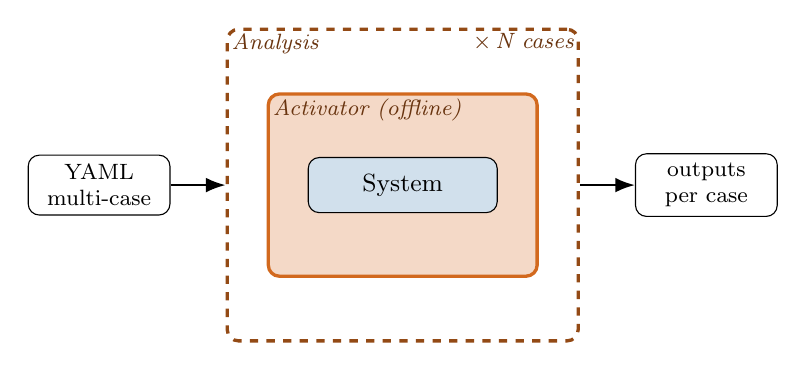
\begin{tikzpicture}[node distance=0.5cm]
  \node[block, fill=devcol!25, minimum width=2.4cm] (sys) {System};

  \begin{scope}[on background layer]
    \node[draw=rescol, very thick, rounded corners, fill=rescol!25,
          fit=(sys), inner xsep=5mm, inner ysep=8mm] (act) {};
  \end{scope}
  \node[font=\footnotesize\itshape, text=rescol!50!black,
        anchor=north west, inner sep=2pt] at (act.north west) {Activator (offline)};

  \node[draw=rescol!70!black, very thick, dashed, rounded corners,
        fit=(act), inner xsep=5mm, inner ysep=8mm] (ana) {};
  \node[font=\footnotesize\itshape, text=rescol!50!black,
        anchor=north west, inner sep=2pt] at (ana.north west) {Analysis};

  \node[block, fill=white, font=\footnotesize, align=center,
        left=0.7cm of ana, minimum width=1.8cm] (yaml) {YAML\\multi-case};
  \node[block, fill=white, font=\footnotesize, align=center,
        right=0.7cm of ana, minimum width=1.8cm] (outs) {outputs\\per case};

  \draw[flow] (yaml) -- (ana);
  \draw[flow] (ana) -- (outs);

  \node[font=\footnotesize\itshape, text=rescol!50!black,
        anchor=north east, inner sep=2pt] at (ana.north east) {$\times$\,N cases};
\end{tikzpicture}

\vspace{0.7cm}
\footnotesize
\begin{tabular}{ll}
\textbf{Analysis} & instantiates an \emph{offline} Activator once per case \\
                  & from a multi-case YAML, and collects per-case outputs \\[2pt]
                  & (the demo Activator's real-time loop never returns, \\
                  & \quad so only the offline variant is usable here) \\
\end{tabular}
\end{frame}

\end{document}
